\documentclass[a4paper,12pt]{article}
\usepackage[utf8x]{inputenc}
\usepackage[czech, english]{babel}
\selectlanguage{czech}
\usepackage[FM, EN, bwtitles, noheader]{tul}
\usepackage[bookmarks]{hyperref}
\usepackage{float}
\usepackage{graphicx}
\usepackage{todonotes}
\presetkeys{todonotes}{inline}{}
\newcommand{\classname}[1]{\texttt{#1}}
\TULphone{+420\,485\,353\,030}
\TULmail{Petr.Jecmen@tul.cz}
\date{September 13, 2013}

\usepackage{listings}
\definecolor{gray}{rgb}{0.4,0.4,0.4}
\definecolor{darkblue}{rgb}{0.0,0.0,0.6}
\definecolor{cyan}{rgb}{0.0,0.6,0.6}
\lstset{
	basicstyle=\ttfamily,
	breaklines=true,
	keywordstyle=\color{darkblue},
	commentstyle=\color{gray},
    frame=trbl,
    rulecolor=\color{black!30},
    xrightmargin=7pt,
	columns=fullflexible,
	showstringspaces=false,
	language=Java
}
\lstdefinelanguage{XML}
{
	morestring=[b]",
	morestring=[s]{>}{<},
	morecomment=[s]{<?}{?>},
	identifierstyle=\color{darkblue},
	keywordstyle=\color{cyan},
	morekeywords={xmlns,version,type}
}

\addto\captionsenglish{
  \renewcommand{\contentsname}
    {Obsah}
}

\begin{document}
\logo
\\\vspace{6pt}
\begin{center}
\large{\bfseries Manuál k softwaru EduApp}
\\\vspace{1pc}
\small{
Ing. Petr Ječmen
\\\vspace{1pc}
Fakulta mechatroniky, informatiky a mezioborových studií\\
Technická Univerzita v~Liberci\\
Studentská 2\\
461 17 Liberec}
\end{center}
\newpage
\section{Přehled}
Po spuštění se hráči zobrazí seznam úrovní. Při prvním spuštění se zobrazí pouze jedna úroveň, další se zobrazí až po dohrání předchozích (stav dohraných úrovní se uchovává i po ukončení aplikace, zatímco stav aktuální úrovně ne).
\begin{figure}[H]
\center{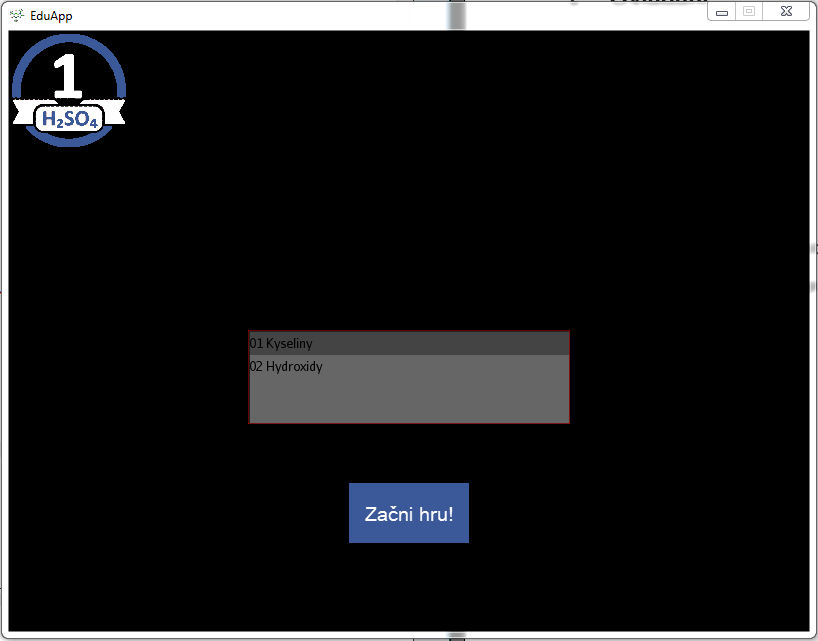
\includegraphics[width=0.5\textwidth]{levelList.png}\\Seznam úrovní}
\end{figure}
Po vybrání (lze myší i klávesnicí) se načte daná úroveň.
\subsection{Ovládání hry}
Hráči se ovládání zobrazí spolu s úvodním textem po načtení úrovně. Následující seznam je ve tvaru "\textbf{akce} klávesa"
\begin{description}
\item[Pohyb] šipky / kliknutí levého tlačítka myši / dotyk stylusem
\item[Akce] mezerník
\item[Seznam úkolů] Q
\item[Slovníček] S
\item[Návrat] Escape
\end{description}
\subsection{Seznam úkolů}
V seznamu se vypisují pouze nedokončené úkoly (ať už ty, ke kterým hráč ještě nedošel nebo ty, které se mu nepodařilo splnit). Ty které uživatel splnil, se nezobrazují. Úkoly, které se nepodařilo splnit, se zobrazí červeným textem a je možné je splnit za pomoci pomocných úkolů.
\begin{figure}[H]
\center{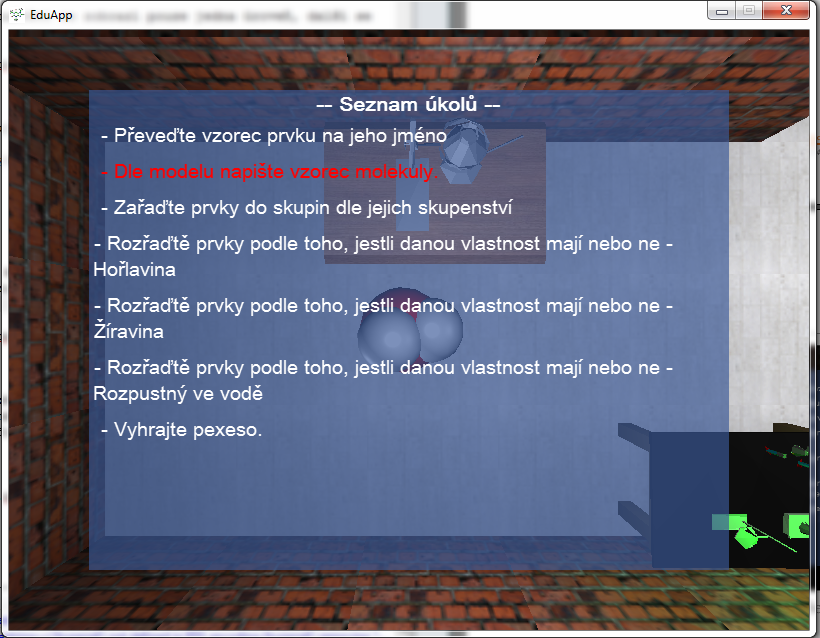
\includegraphics[width=0.5\textwidth]{questList.png}\\Seznam úkolů pro chemii}
\end{figure}
\subsection{Slovníček}
\begin{description}
\item[Ikony] Libovolvý obrázek, slouží pro indikaci nějaké vlastnosti (např. toxicita, rozpustnost atd.)
\item[Text] Lze prezentovat víceméně libovolný text (formát je nadpis a pod ním text)
\item[Odkazy] na webové stránky, kde lze nalézt další informace (odkazy jsou aktivní, tzn. že po kliknutí na ně se otevře daná stránka)
\end{description}
\begin{figure}[H]
\center{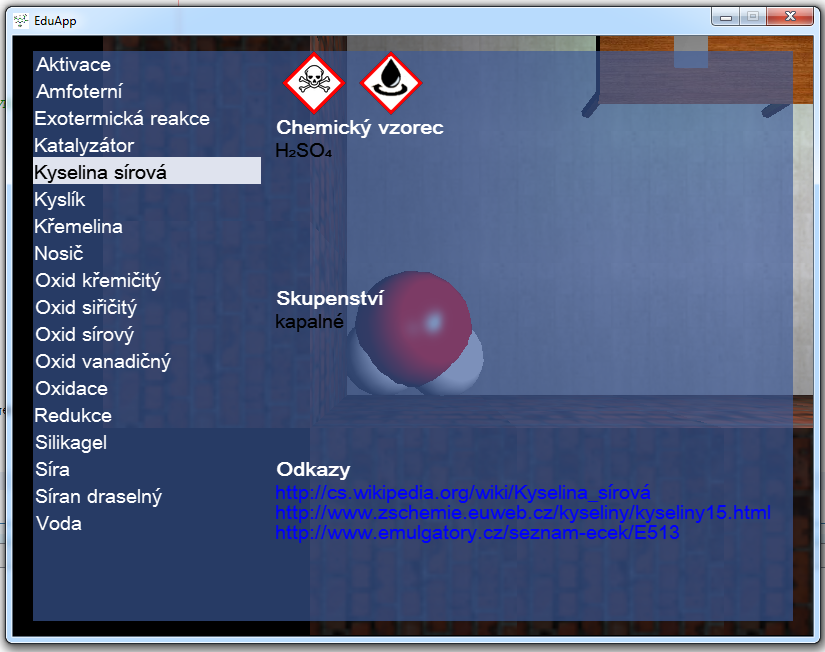
\includegraphics[width=0.5\textwidth]{dictionary.png}\\Slovníček pro chemii}
\end{figure}
\newpage
\section{Úkoly}
U většiny úkolů se uživatel kromě finálního výsledku úkolu (splněno / nesplněno) dozví i to, co bylo špatně a co správně (typicky prezentováno zeleným / červeným podbarvením). Na každý úkol je pouze jeden pokus, v případě špatné odpovědi nebo přerušení otázky za pomoci klávesy Esc je nutno úkol splnit za pomoci pomocné otázky.
\subsection{Text dle modelu}
Hra používá panel aplikace JMol (http://jmol.sourceforge.net/) pro prezentaci chemických modelů a struktur. Úkol tedy spočívá v tom, že se uživateli prezentují modely a on na základě nich vyplní nějaký text (typicky vzorec nebo název struktury).
\begin{figure}[H]
\center{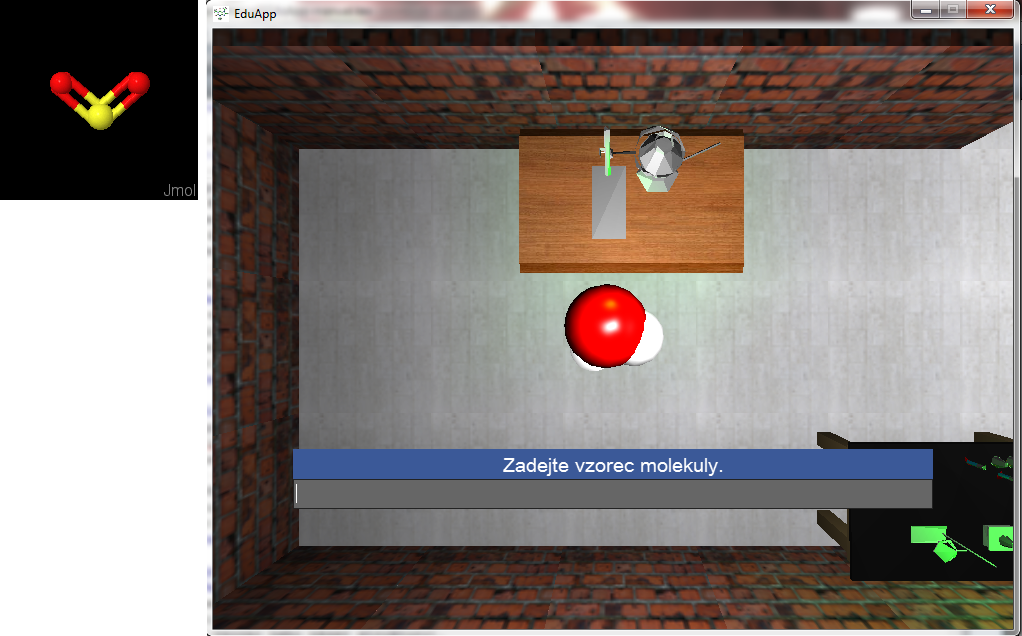
\includegraphics[width=0.5\textwidth]{questJmol.png}\\Úkol text dle modelu}
\end{figure}
\subsection{Převod}
Hráč má za úkol převést daný text (např. vzorec) na jinou reprezentaci (např. název).
\begin{figure}[H]
\center{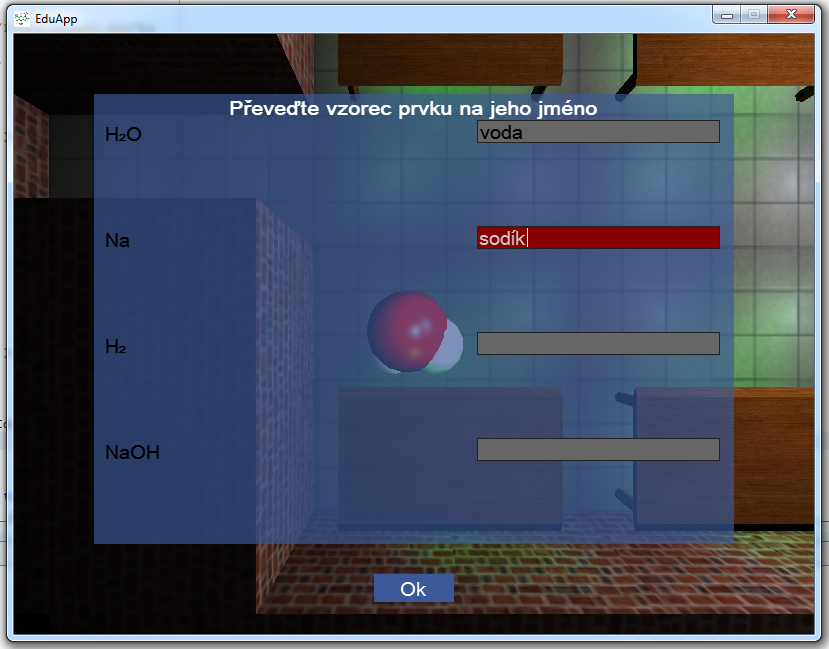
\includegraphics[width=0.5\textwidth]{questConversion.png}\\Úkol převod}
\end{figure}
\subsection{Rozřazování do skupin}
Hráči je prezentováno několik skupin a sada předmětů, které musí správně zařadit. Předmět může patřit do více skupin, v tom případě je jedno, do které skupiny ho hráč zařadí, pouze k ní musí náležet.
\begin{figure}[H]
\center{\includegraphics[width=0.5\textwidth]{questGroups.png}\\Úkol rozřazení do skupin}
\end{figure}
\subsection{Pexeso}
Jedná se o klasické pexeso, kdy uživatel musí hledat páry hodící se k sobě. Lze hrát bez limitu nebo s limitem času nebo počtu tahů. Spojuje se typicky text a obrázek, lze ale realizovat i jiné varianty.
\begin{figure}[H]
\center{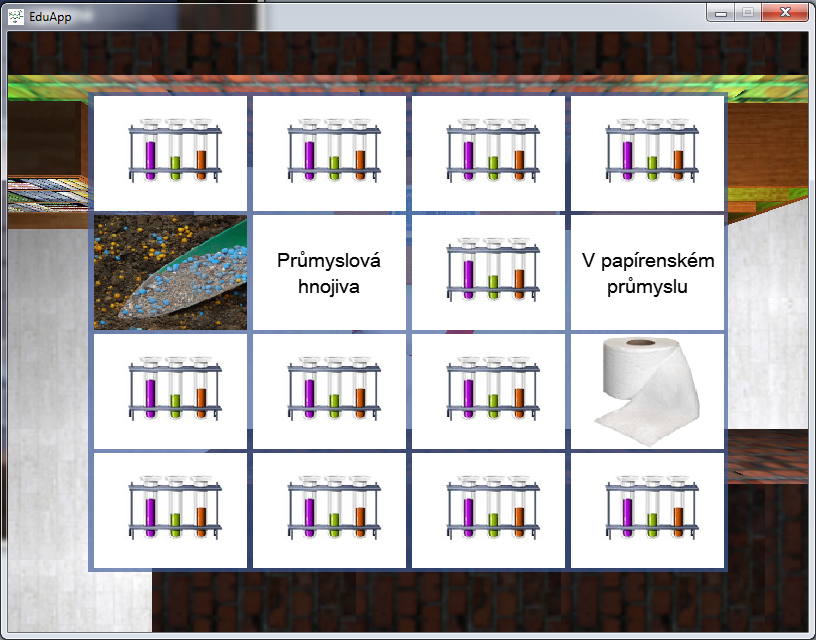
\includegraphics[width=0.5\textwidth]{questPexeso.png}\\Úkol pexeso}
\end{figure}
\subsection{Otázka}
Hráč musí odpovědět na zadanou otázku. Je možné vyžadovat přesnou shodu (řeší se velká / malá písmena, vhodné např. pro vzorce) nebo se může vyžadovat pouze shoda obsahu (bez rozlišení malých / velkých písmen).
\subsection{Otázka s webovou stránkou}
Jedná se o stejný typ úkolu jako obyčejná otázka, pouze se hráči otevře webová stránka, na které by měl danou informaci dohledat.
\subsection{Doplnění rovnice}
Tento úkol je primárně určen pro chemii, lze ho ale použít i pro jiné obory. Jedná se o sestavení rovnice (či rovnic) z daných předmětů.
\begin{figure}[H]
\center{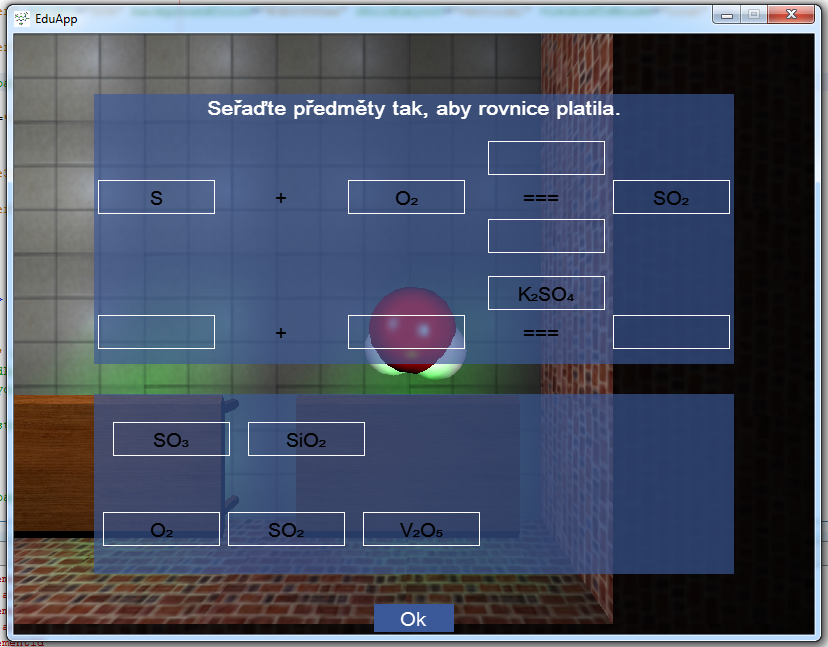
\includegraphics[width=0.5\textwidth]{questEquation.png}\\Úkol rovnice}
\end{figure}
\subsection{Vybírání vlastnosti látky}
Uživatel musí zadat hodnotu vybraných vlastností dané látky.
\subsection{Doplnění textu slovy}
Zobrazí se text, ve kterém jsou vynechány některá slova. Uživatel dostane k dispozici několik slov, která musí správně umístit do textu.
\subsection{Sestavení postupu}
Uživatel dostane k dispozici sadu kroků, které po správném seřazení reprezentují postup něčeho.
\subsection{Přiřazení název popis}
Uživatel musí připojit správný popis k danému slovu.
\subsection{Výběr odpovědi dle otázky}
Klasický výběr odpovědi z více možností na základě zadané otázky.
\begin{figure}[H]
\center{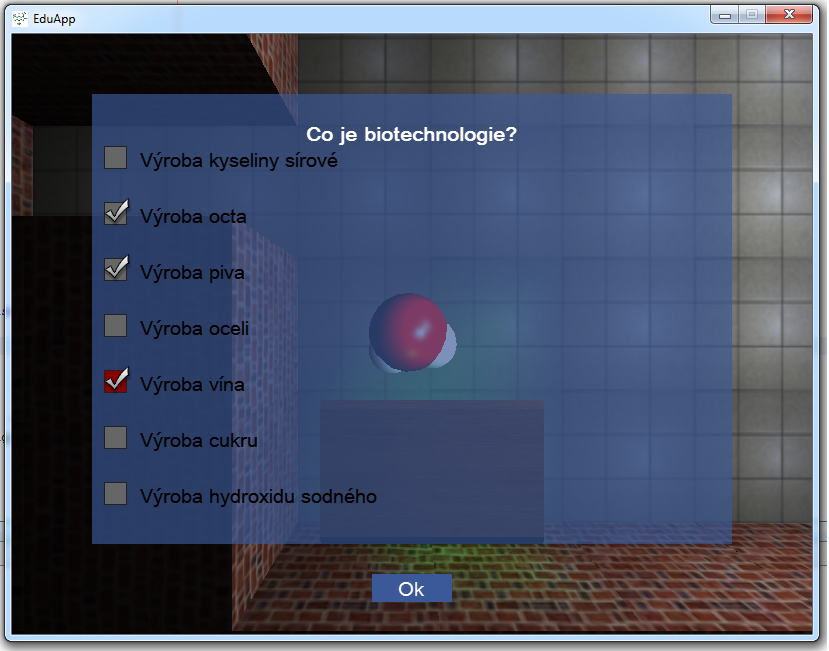
\includegraphics[width=0.5\textwidth]{questMultiAnswer.png}\\Úkol výběr odpovědi}
\end{figure}
\subsection{Pomocné úkoly}
Pomocné úkoly jsou ve formě otázek. Měly by představovat jakousi záchranu v případě, že se hráči nepodaří splnit nějaký úkol. Typicky by se mělo  jednat o otázku, na kterou musí hráč odpověď dohledat někde "dále" (např. ji lze nalézt na stránce uvedené v odkazech k danému předmětu ve slovníčku). Tento úkol nelze nesplnit (při přerušení se nic neděje, hráč se k ní může vrátit kdykoliv později).
\newpage
\section{Data úrovně}
V případě, že by jste chtěli vytvářet vlastní úroveň, je nutné dodat následující data.\\
\begin{description}
\item[Design úrovně] Alespoň hrubý nárys, jak si představujete prostředí (rozložení předmětů a úkolů, vzhled úrovně apod.)
\item[Texty] úvodní text (zobrazí se po načtení úrovně), závěrečný text (zobrazí se po dokončení všech úkolů)
\item[Úkoly] seznam úkolů - typ úkolu a data úkolu (možnosti úkolů viz. seznam) 
\item[Slovníček] "strukturovaná" data, která chcete, aby se hráč mohl naučit (např. vlastnosti jako hořlavost, toxicita apod., které se dají prezentovat za pomoci ikon, popisný text a odkazy na web, kde lze nalézt další informace)
\end{description}
\end{document}